% Frame 29: Third Assignment
\begin{frame}
    \frametitle{Third Assignment Dataset}
    For the third assignment we are implementing a transformer which is 
    trained on the MNIST Dataset. The MNIST dataset has:
    \begin{itemize}
        \item 60,000 training images
        \item 10,000 testing images
        \item 10 classes
        \item 28x28 pixels each image
    \end{itemize}
    \begin{figure}
        \centering
        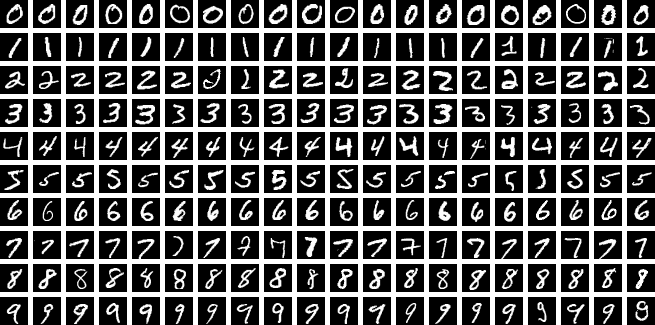
\includegraphics[height=0.4\textheight]{media/3rdAssignment/MNIST_dataset_example.png}
        \vspace{-0.35cm}
        \caption{MNIST Dataset}
    \end{figure}
\end{frame}

% Frame 30: Simple Transformer
\begin{frame}
    \frametitle{Simple Transformer}
    The simple transformer revolves around a CNN encoder/decoder architecture. 
    It is comprised of:
    \begin{itemize}
        \item Encoder: Extracts the latent representation of the input image
        \item Transformer: Modifies that representation to approximate the next
        image in the sequence through the Dataset Dictionary class.
        \item Decoder: Takes the modified representation and generates an image
        from it.
    \end{itemize}
\end{frame}

% Frame 31: Simple Transformer Architecture
\begin{frame}
    \frametitle{Simple Transformer}
    Encoder: Creates the latent representation 
    \begin{itemize}
        \item 2 Convolutioanl Layers
        \item 2 ReLU Activation Functions
        \item 1 Flatten Layer
    \end{itemize} 
    Transformer: Modifies the latent representation
    \begin{itemize}
        \item 2 Linear Layers
        \item 1 ReLU Activation Function
    \end{itemize}
    Decoder: Generates the image from the modified representation
    \begin{itemize}
        \item 1 Linear Fully Connected Layer
        \item 2 Transpose Convolutional Layers
        \item 2 Activation Functions (ReLU and Tanh)
    \end{itemize}
\end{frame}

% Frame 32: Simple Transformer Results
\begin{frame}
    \frametitle{Simple Transformer Output Examples}
    \begin{figure}
        \centering
        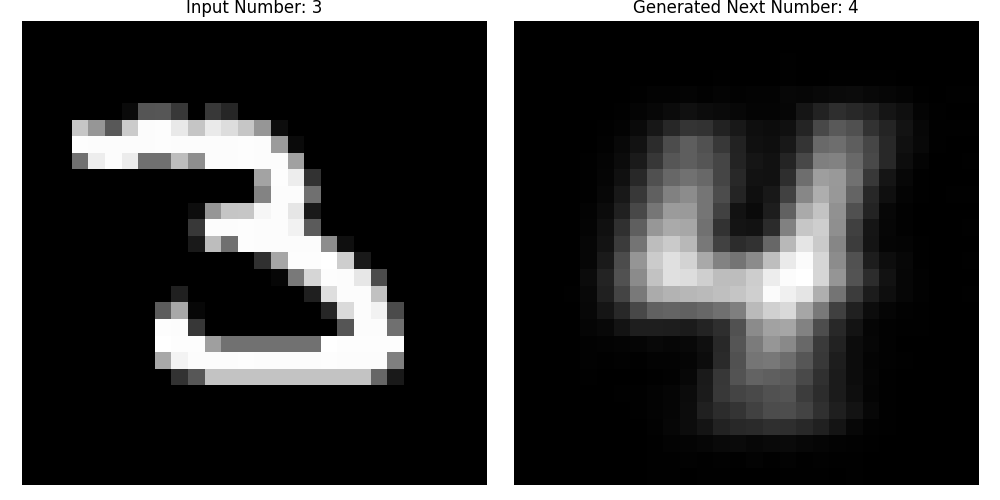
\includegraphics[height=0.35\textheight]{media/3rdAssignment/Figure_3.png}
        \vspace{-0.35cm}
        \caption{Good Example}
    \end{figure}
    \vspace{-0.35cm}
    \begin{figure}
        \centering
        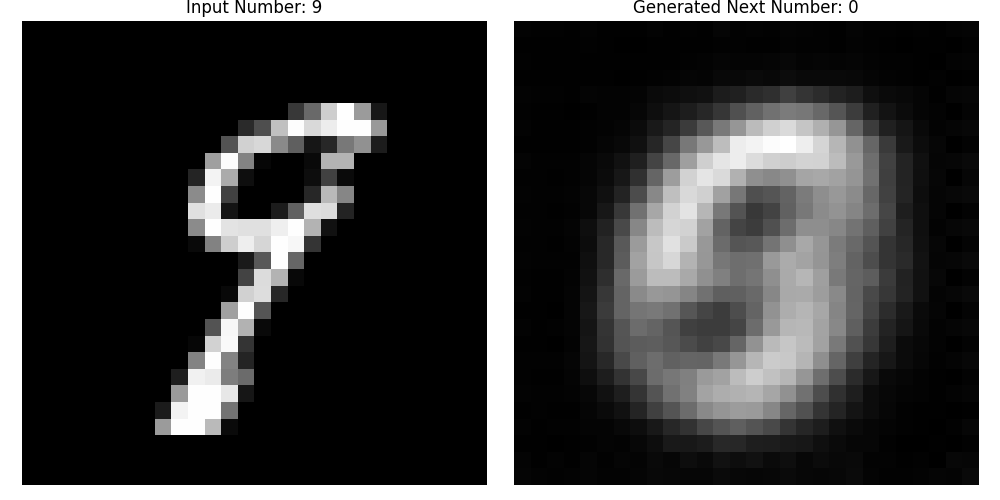
\includegraphics[height=0.35\textheight]{media/3rdAssignment/Figure_4.png}
        \vspace{-0.35cm}
        \caption{Bad Example}
    \end{figure}
\end{frame}

% Frame 33: Seft-Attention Transformer 
\begin{frame}
    \frametitle{Self-Attention Transformer}
    The self-attention transformer differs from the simple transformer only in
    the transformer class. Here:
    \begin{itemize}
        \item Multi-Head Attention Layer
        \item Feed Forward bundle of:
        \begin{itemize}
            \item 2 Linear layers
            \item 1 ReLU Activation function
        \end{itemize}
        \item 2 Normalization layers
    \end{itemize}
\end{frame}

% Frame 34: Simple vs Self-Attention Transformer Results
\begin{frame}
    \frametitle{Simple vs Self-Attention Transformer}
    \begin{figure}
        \centering
        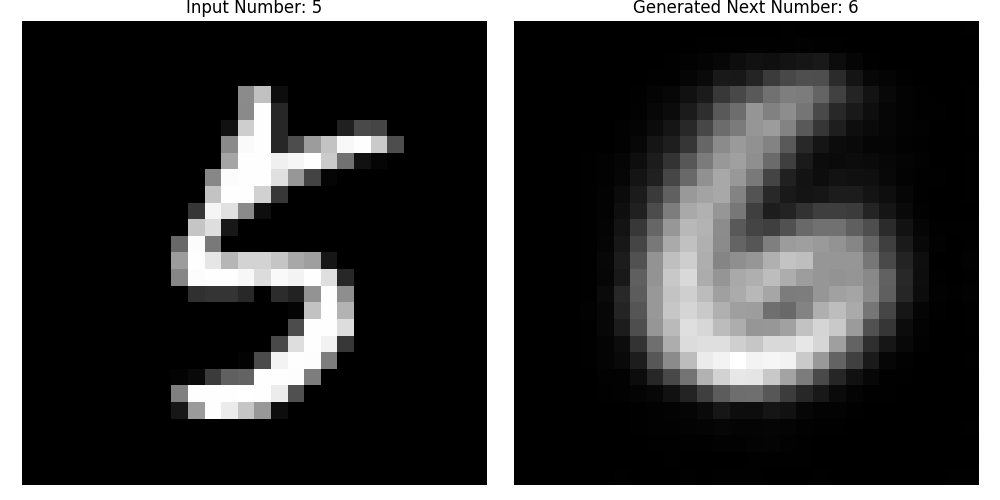
\includegraphics[height=0.35\textheight]{media/3rdAssignment/Simple.png}
        \vspace{-0.35cm}
        \caption{Simple Transformer}
    \end{figure}
    \vspace{-0.35cm}
    \begin{figure}
        \centering
        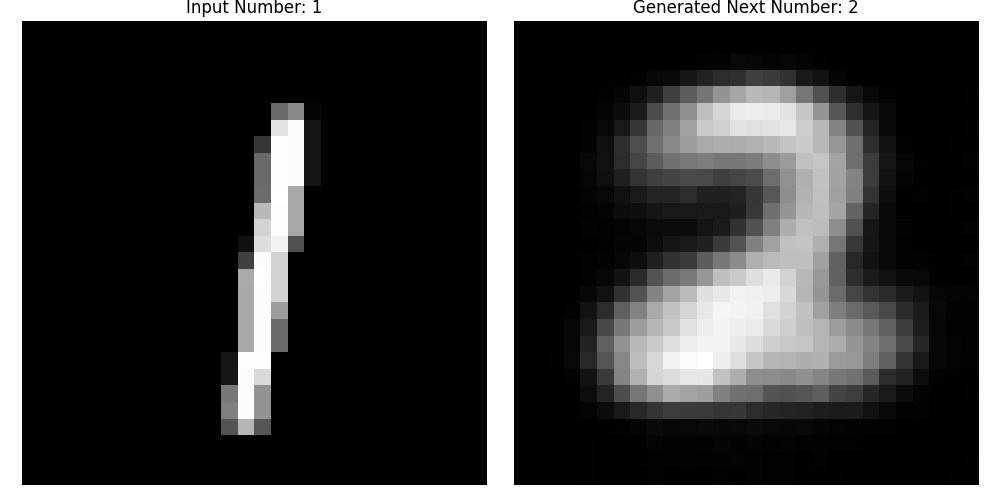
\includegraphics[height=0.35\textheight]{media/3rdAssignment/Self_attention.png}
        \vspace{-0.35cm}
        \caption{Self-Attention Transformer}
    \end{figure}
\end{frame}

% Frame 35: PCA
\begin{frame}
    \frametitle{PCA}
    \begin{columns}
        \begin{column}{0.7\textwidth}
            PCA (Principal Component Analysis) is a dimensionality reduction technique that we
            used in order to reduce the $28 \times 28=784$ dimensions into principle components.
            The procedure:
            \begin{itemize}
                \item Normalization to range [0,1]
                \item Reduce dimensionality via PCA
                \item Select digit to generate
                \item Add random noise (Perturbation)
                \item Inverse transform the PCA
                \item Display the image
            \end{itemize}
        \end{column}
        \begin{column}{0.3\textwidth}
            \begin{figure}
                \centering
                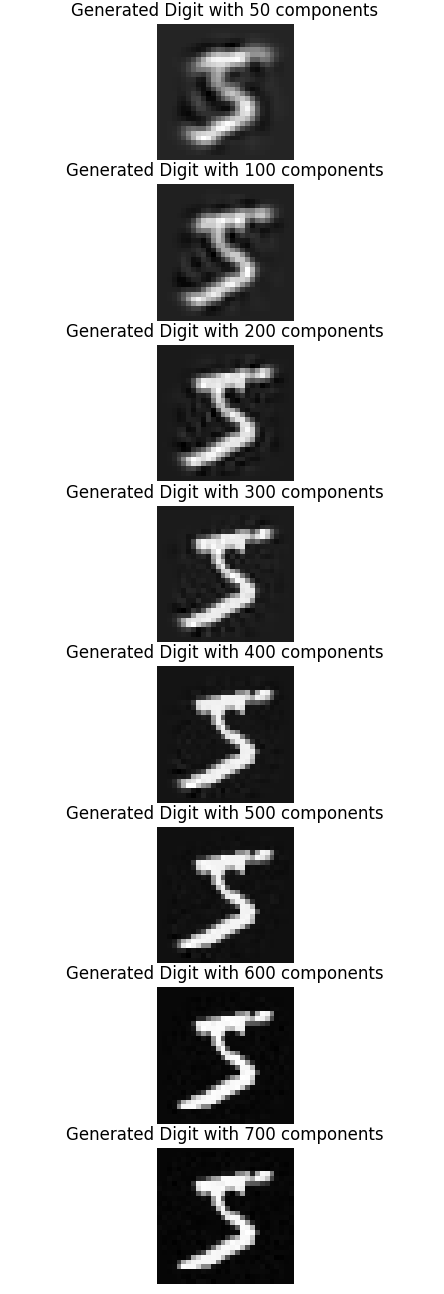
\includegraphics[height=0.8\textheight]{media/3rdAssignment/PCA_components.png}
            \end{figure}
        \end{column}
    \end{columns}
\end{frame}

% Frame 36: CNN Interpreter and Custom Test Set vs MNIST Test Set
\begin{frame}
    \frametitle{Custom Test Set vs MNIST Test Set}
    A CNN Neural network the same as the one used in the first assignment tested on the
    MNIST test set and a custom test set. Only 1 Epoch needed.\\
    
    \vspace{0.3cm}
    \tiny

    \begin{columns}
        \begin{column}{0.5\textwidth}
            \textbf{MNIST Test Set}
            \begin{itemize}
                \item \textbf{Average loss}: 0.0454
                \item \textbf{Accuracy}: 98.41\%
            \end{itemize}
            \textbf{Per-class accuracy}:
            \begin{itemize}
                \item 0: 99.29\%
                \item 1: 99.12\%
                \item 2: 98.84\%
                \item 3: 99.50\%
                \item 4: 97.76\%
                \item 5: 96.64\%
                \item 6: 98.43\%
                \item 7: 98.05\%
                \item 8: 98.87\%
                \item 9: 97.32\%
            \end{itemize}
        \end{column}
        \begin{column}{0.5\textwidth}
            \textbf{Custom Test Set}
            \begin{itemize}
                \item \textbf{Average loss}: 0.2716
                \item \textbf{Accuracy}: 96.00\%
            \end{itemize}
            \textbf{Per-class accuracy}:
            \begin{itemize}
                \item 0: 88.89\%
                \item 1: 90.00\%
                \item 2: 100.00\%
                \item 3: 90.00\%
                \item 4: 90.00\%
                \item 5: 100.00\%
                \item 6: 100.00\%
                \item 7: 100.00\%
                \item 8: 100.00\%
                \item 9: 100.00\%
            \end{itemize}
        \end{column}
    \end{columns}
\end{frame}

